\section{Communicating with the satellite}

\begin{figure}
  \begin{center}
    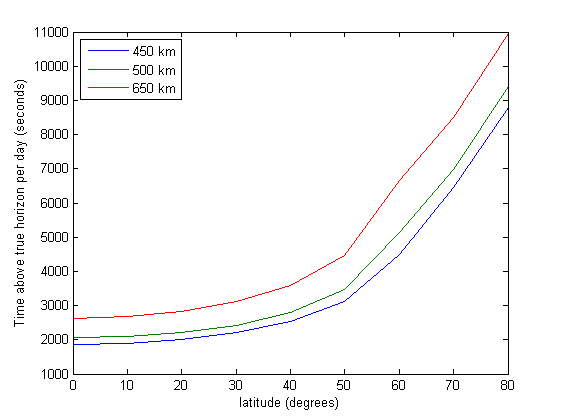
\includegraphics[width=1.0\textwidth]{Figures/accesstid450_500_650horizont}
  \end{center}
  \caption[LOS for 450 and 650]{Time above the horizon for a satellite with altitude $h=450km$, $h=500km$ and $h=650km$ as a function of ground station latitude}
  \label{fig:access_horizon}
\end{figure}

\begin{figure}
  \begin{center}
    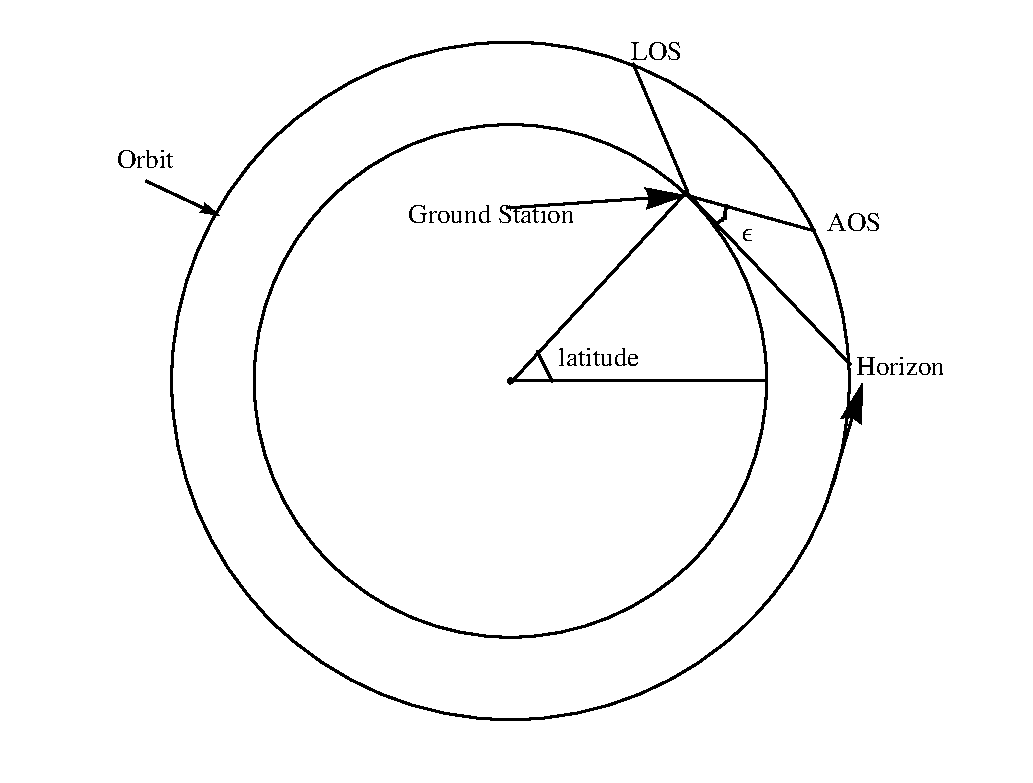
\includegraphics[trim = 5mm 30mm 5mm 0mm, clip, width=0.8\textwidth]{Figures/groundstation_satellite_geometry}
  \end{center}
  \caption[Ground station satellite geometry]{Illustration of geometry between a ground station and a satellite}
  \label{fig:ground_station_satellite_geometry}
\end{figure}

Since we don't know when the satellite will be launched we don't know the exact orbit. The project manager, Roger Birkeland, told us that we can assume the orbit will  have a height above the Earth somewhere between 450km and 650km and inclination of 98 degrees.

The height above the earth dramatically changes the time the satellite is seen by the ground station, see Fig. \ref{fig:access_horizon}. The signal will be weaker when the satellite is further away, it is therefore necessary to increase the minimum elevation angle $\epsilon$, see Fig. \ref{fig:ground_station_satellite_geometry}, to maintain SNR.  Previous work\cite{antennemaster,bildemaster} has calculated the minimum elevation angle, for a ground station here in Trondheim, for satellites with different altitudes and found that these effects cancel each other out. In the following we'll assume that the altitude is 500 km and the minimum elevation angle is 28 degrees.

\begin{figure}
  \begin{center}
    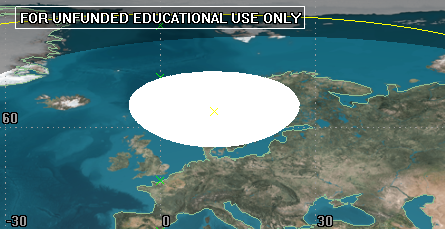
\includegraphics[width=0.8\textwidth]{Figures/ntnu_footprint}
  \end{center}
  \caption[NTNU footprint]{NTNU ground station range}
  \label{fig:ntnu_range}
\end{figure}

The result of this is that the ground station can communicate with the satellite whenever the ground track is inside a rough circle centered on the ground station, see Fig. \ref{fig:ntnu_range} for the estimated "range" of the ground station at Gløshaugen operating with these constraints. The efficiency of a network of ground stations is reduced when the ranges overlap, so to have a sufficient network the nodes must be geographically far apart. In this case the ground stations must be more than 1600 km apart to have maximum efficiency.

The Gløshaugen ground station will on average be able to communicate with the satellite 520 seconds per day. With a bit rate of 9600 bps 600kB can be downloaded per day on average.

\subsection{Other ground stations}
\begin{figure}
  \begin{center}
    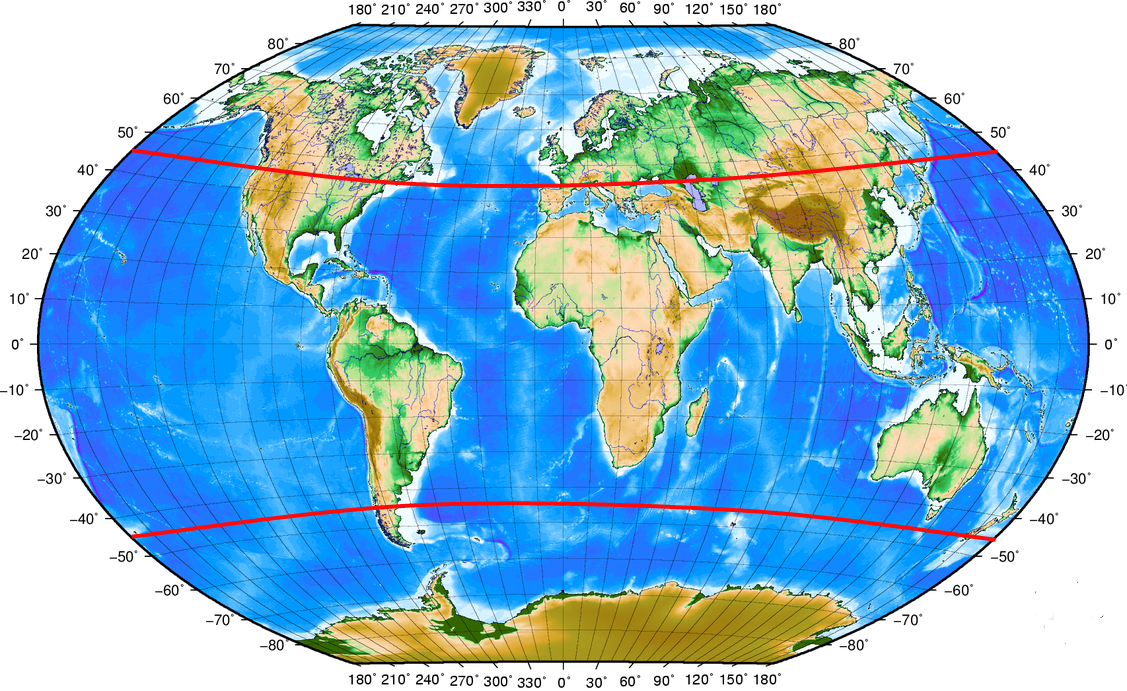
\includegraphics[width=0.9\textwidth]{Figures/verdenskart}
  \end{center}
  \caption[world]{Map of the World}
  \label{fig:world}
\end{figure}

Fig. \ref{fig:access_horizon} shows that the access time for a (near) polar satellite is almost latitude independent for ground stations at latitudes below 45 degrees. The access times of a ground station those low latitudes are about about 280 seconds/day, i.e. half the duration we get here in Trondheim. For higher latitudes the access time increases dramatically. And the average access time for a ground station in Longyearbyen (78N) is in fact as high as 1300 seconds/day.
